\chapter{Introduction}
\label{chap:intro}
\minitoc

The use of physiological parameters has proven to be highly effective in a wide variety of medical settings, which was enhanced with the wide adoption of oxygen saturation monitoring~\cite{Williams2022}. This demonstrates how informative this physiological parameter can be in clinical decision making. Similarly there have been many advancements in intra-operative monitoring technologies particularly in the neurosurgical field~\cite{Raith2020}. As yet, however, there have been no spatially-resolved tissue oxygen saturation ($StO_2$) visualisation methods that could be easily integrated into clinical use. 

The work in this thesis aims to provide a hyperspectral imaging (HSI) system that is easy to integrate by providing a fully sterile alternative to traditional calibration steps, evaluating some key analytical tissue models for $StO_2$ extraction, and some initial exploration into applying this to HSI data for neurosurgical applications. 

This chapter presents some clinical context of brain tumours (Section \ref{sec:braintumours}) and aneurysms (Section \ref{sec:aneurysms}) for which this research is targeted alongside the current, relevant, available clinical adjuncts. This is followed by a description of oxygen saturation (Section \ref{sec:oxygensat}) and some key existing technologies to compute this and their limitations (Section \ref{sec:stateofart}). Finally, the structure of this thesis is presented in Section \ref{sec:thesisoutline}.

% This work aims to use a Hyperspectral Imaging (HSI) camera to extract semantic and physiologically relevant data in real-time during neuro-oncological surgery. These data are expected to aid decision-making, thereby reducing cognitive workload for the surgeons without compromising patient outcomes. The following introduction summarises the fundamentals of brain tumours and current operating practice.  This is followed by a summary of Hyperspectral Imaging, key data post-processing steps, and an outline of the thesis.
%
\section{Brain tumours}\label{sec:braintumours}
Brain tumours arise as a subset of the collection of diseases termed cancer. Whilst there can be hereditary contributions to cancers, they can also occur due to damage in the DNA caused by exposure to certain environmental risk factors such as tobacco smoke or ultraviolet radiation~\cite{WorldHealthOrganisation2023}. Cancers are characterised by an uncontrolled multiplication of unspecialised cells; these regions of growth are termed tumours~\cite{WorldHealthOrganisation2023}. Symptoms of brain tumours can range from headaches and nausea to changes in personality and paralysis~\cite{NationalHealthService2023}. With only 4 in 10 of those aged 15-44 years old diagnosed with a brain tumour surviving the disease for at least 10 years, and the number dropping to 1 in 10 when all age ranges are considered, these cancers have significant impact and require improved understanding and treatment~\cite{CancerResearchUK2023}. For this reason, we aim to provide more intra-operative information to aid surgical guidance for improved treatment of brain tumours using hyperspectral imaging. 

\subsection{Categorising tumours} 
Tumours can fall into one of the two categories: malignant or benign. A malignant tumour can invade local tissues or some cells can travel through the blood stream and cause tumours in other regions of the body, labelled metastatic tumours. In contrast a benign tumour will not invade local or distal tissues, and, unlike malignant tumours, are likely not to grow back if removed~\cite{Institute2021}. The likelihood of a tumour to grow and spread determines its grade, which can range from Grade 1 (rarely spread and can generally can be cured by surgery) to Grade 4 (grow and spread very quickly and usually cannot be cured)~\cite{Institute2023}. Unlike other regions of the body, even benign tumours in the brain can be life-threatening. A brain tumour can grow and press on regions of the brain causing those areas to stop working leading to a range of symptoms. This is true for both primary brain tumours, that originate in the brain, and metastatic brain tumours, that originate elsewhere in the body~\cite{Institute2021}.

The type of tumour and it's impact is determined by the region of brain it affects. There are three main sections of the brain which each control different aspects of human functioning. Some examples are shown in Figure \ref{fig:anatomybrain} and include the cerebrum, which is the largest part of the brain and controls thinking, learning, problem solving, emotions, speech, reading, writing, and voluntary movement; the cerebellum controls movement, balance, and posture; and the brain stem which connects the brain to the spinal cord and controls breathing, heart rate, and the nerves and muscles used to see, hear, walk, talk, and eat~\cite{Institute2023}.
\begin{figure}[ht]
    \centering
    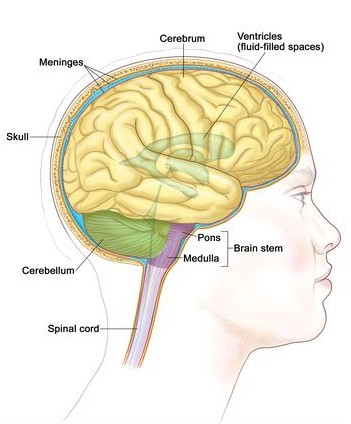
\includegraphics[width=0.55\textwidth]{brainanatomy.jpg}
    \caption{Depiction of some key regions of the brain reproduced from~\citenum{Institute2023}.}
    \label{fig:anatomybrain}
\end{figure}
There are also different types of brain cells in which the tumour can originate. The brain contains many neurones which transport the electrical signals that allow the brain to operate. These are surrounded by glial cells, of which there are different types which each play a role in supporting and protecting the neurones~\cite{TheBrainTumourCharity2023}. The main types are astrocytes, oligodendrocytes and ependymal cells. When the tumour originates in glial cells it is termed a glioma with subcategories corresponding to each type of glial cell. Astrocytomas, originating in astrocytes, are the most common gliomas with the different grades given different names such as Grade 4 astrocytoma named glioblastoma multiforme~\cite{BrainTumourResearch2023}. Similarly, oligodendrogliomas originate from oligodendrocytes, and ependymomas originate from ependymal cells~\cite{TheBrainTumourCharity2023}. %include meningioma lymphoma medulloblastoma adenoma \\

There are over 130 types of brain tumours as classified by the World Health Organisation (WHO) and differ in terms of which type of cell they originate in, their grade, and which part of the brain they affect.

\subsection{Current treatments}\label{sec:introtumourtreatments}
Initially or if no other treatment options are possible, the symptoms of a brain tumour can be treated without treating the tumour itself, for example anti-sickness medication to treat the nausea. The treatment plans are determined based on a number of factors which include the type, location, and grade of the tumour as well as the patient's overall health~\cite{NationalHealthService2023}. Surgery is a preferred treatment where possible as it is possible to remove a large proportion, if not all, of the tumour with this method. In cases where the full tumour may not be removed, such as when there is a significant infiltration zone into surrounding healthy tissue where the border of the tumour is challenging to identify, this may be followed up with radiotherapy or chemotherapy. These treatment options can also be used separately when surgery is not an option~\cite{MacmillanCancerSupport2019}. 

Neurosurgical resection aims for maximum safe resection of the tumour which balances a high extent of resection while preserving functional regions of brain as improved resection is linked to improved patient outcomes~\cite{Chanbour2022}. To this end a variety of techniques can be employed to improve resection. These include: a surgical microscope which enables clear visualisation of the surgical field, neuronavigation which allows registration of a probe against an MRI, awake or asleep sub-corticol mapping to allow identification of eloquent areas of brain, in some cases fluorescence imaging using 5-aminolevulinic acid (5-ALA) or indocyanine green (ICG) can be used for tumour localisation, and microvascular doppler (MVD) or ICG can be used for tumour vessel localisation~\cite{Chanbour2022, Catapano2018}.

Whilst these these adjuncts have improved the quality of tumour resection, they are associated with some limitations~\cite{Chanbour2022}. Neuronavigation reduces in accuracy as the anatomy changes throughout a procedure, known as brain shift. Whilst this can be counteracted using intra-operative MRI, this disrupts surgical workflow and has large associated costs~\cite{Chanbour2022}. Sub-cortical mapping allows identification of eloquent regions of brain, however this does not provide a spatially-resolved tumour boundary and carries risks of intraoperative seizures or postoperative emotional distress~\cite{Chanbour2022}. Label-based methods such as fluorescence utilising 5-ALA or ICG can be effective but are limited by the label behaviour and the type of tumour in which it is effective~\cite{Chanbour2022}. For example, fluorescence imaging has been shown to have limited application in low grade glioma resections due to the low aggregation of fluorophore in these less aggressive tumours~\cite{Belykh2023, Kiesel2021, Jaber2019}. Vessel localisation may also be effective with MVD or ICG displaying the flow of blood, however this is unable to quantify the oxygen saturation of this blood or verify the oxygen transfer into tissues which introduces an element of subjectivity into tissue viability assessment. Even the widely adopted surgical microscope can be associated with operator fatigue and its maneuverability is limited by its size~\cite{Alamer2023}. Exoscopes have been proposed to address these challenges, however these are associated with potential learning curves for new users~\cite{Alamer2023}.

Where these techniques have been used they have improved patient outcomes while demonstrating some key features that aid in surgical integration. The introduction of real-time visualisation with a high spatial resolution from the surgical microscope has lead to improvements in maximal safe tumour resection~\cite{Alamer2023}. For this reason, fluorescence imaging and ICG have been incorporated into such devices to make use of these properties. These techniques illustrate the importance of tools that enable accurate distinction between healthy and cancerous tissues for safe resection~\cite{Belykh2023}. These features are all present in intra-operative MRI, however its limited adoption draws attention to the importance of ensuring technological advancements integrate well with the surgical workflow. The detrimental impact of brain shift on the quality of neuronavigation demonstrates the importance of real-time evaluation to ensure all information presented is accurate for the anatomy onto which it is applied~\cite{Alamer2023}. The importance of vessel visualisation is also seen in the applications of ICG where this allows for tumour feeding and peritumour vessels to be visualised enabling improved retention of normal anatomy post-resection~\cite{Catapano2018}. This demonstrates the need for real-time, spatially-resolved, visualisation of tumour boundaries and vascularisation intra-operatively. Whilst many existing clinical adjuncts address subsets of these properties, HSI presents potential to address all of these.  

\section{Brain aneurysms}\label{sec:aneurysms}
Another key set of conditions addressed by neurosurgery include brain aneurysms. These are a subset of all aneurysms which are balloon-like abnormal dilatations in a vessel wall due to a weakness caused by high blood pressure, smoking, or genetic predisposition~\cite{NationalHealthService2022}. Most aneurysms will only have significant symptoms on rupturing which is called a subarachnoid haemmorhage and can cause extensive brain damage as well as blinding headaches, sickness, or pain looking at light~\cite{NationalHealthService2022} with approximately 500,000 people dying annually~\cite{Toth2018}. We aim to aid surgical guidance in treatment of aneurysms using hyperspectral imaging. 

\subsection{Current treatments}\label{sec:introaneurysmtreatments}
Treatment of unruptured aneurysm is determined by risk of rupture, size, and location in the brain. If the aneurysm is considered to have a low risk of rupture, treatment may focus on limiting risk factors~\cite{NationalHealthService2022}. In ruptured aneurysms or those at higher risk of rupturing, however, treatment is primarily surgical in the form of clipping or endovascular procedures depicted in Figure \ref{fig:aneurysmtreatment}. The former involves the placement of a metal clip over the opening to prevent further blood flow into the aneurysm~\cite{TheBrainFoundation2023}. Endovascular procedures can include coiling to encourage clotting in the aneurysm to prevent further blood flow, which can be combined with further devices including stents to hold the coil in place~\cite{TheBrainFoundation2023}. The final endovascular technique is flow diversion achieved by placing a cylindrical tube (similar to a stent with a tighter weave) in the vessel over the aneurysm opening to allow normal blood flow~\cite{TheBrainFoundation2023}. 
\begin{figure}[h]
    \centering
    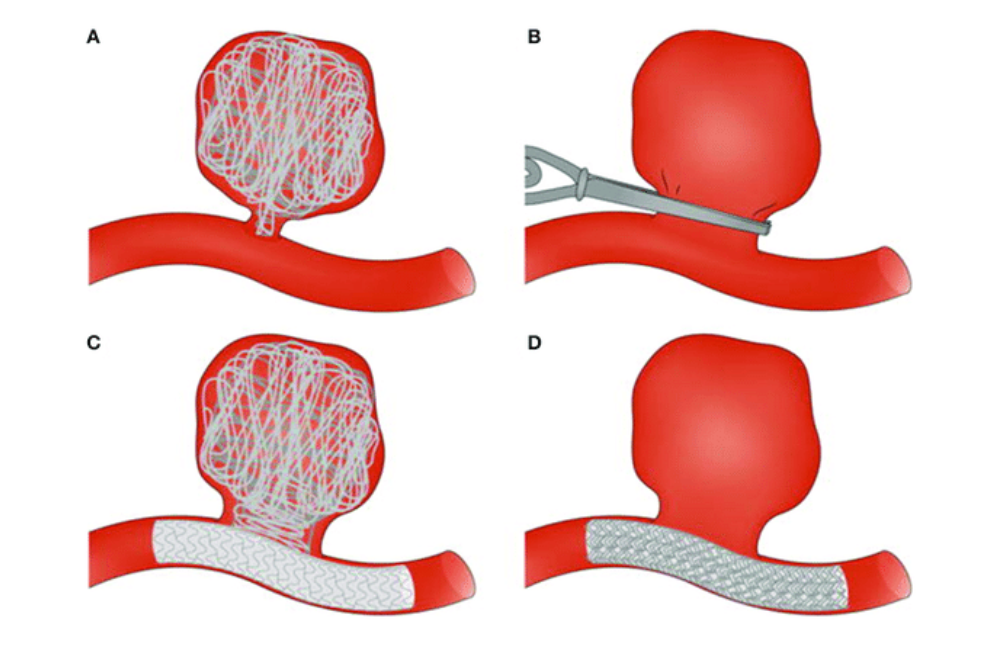
\includegraphics[width=0.9\textwidth]{Aneurysm-treatments.png}
    \caption{An illustration of some key surgical treatment methods for brain aneurysms reproduced from~\citenum{TheBrainFoundation2023} where the technique depicted by A is coiling, B is clipping, C is coiling combined with a stent, and D is flow diversion.}
    \label{fig:aneurysmtreatment}
\end{figure}
Whilst these treatment methods are often very effective, incomplete aneurysm occlusion can lead to rupture at a later date with the extent of occlusion being linked to the likelihood of this occurring~\cite{Toth2018}. For this reason blood flow is often assessed intra-operatively using digital subtraction angiography (DSA), MVD, or ICG~\cite{Norat2019}. DSA is produced by subtracting an X-ray image taken without a contrast agent from one taken with a fluorescent contrast agent to visualise only the vessels in the field of view~\cite{Radiopia2022}. This can be done intra-operatively to visualise the blood flow, however the gold-standard for determining quality of aneurysm occlusion is a post-operative DSA~\cite{Marbacher2020}. DSA cannot be used continuously intra-operatively due to the changing geometry, the complex procedure for DSA aquisition, and the radiation dose risk~\cite{Radiopia2022, Derdeyn1999}. ICG provides a real-time alternative to DSA, however it also requires a fluorescent dye and is of lower precision~\cite{Norat2019, Anania2023}. MVD is also able to determine if full occlusion has occurred intra-operatively and has the advantage of not requiring a labelling agent, however this technique is highly subject to angle and depth~\cite{Anania2023}. Additionally, temporary clipping of healthy vessels can be used to control intra-operative bleeding, however this may lead to cerebral ischaemia where tissues have limited access to oxygenated blood~\cite{Doron2022}. 

Similarly to those in Section \ref{sec:introtumourtreatments}, the advantages of the current clinical adjuncts provide valuable information of the desirable features in technology to aid aneurysm treatment. DSA, ICG and MVD all demonstrate the desirability of spatially-resolved evaluation technique. DSA and MVD highlight the importance of accounting for changing geometry or imaging position, while ICG draws attention to the advantage of label-free techniques. While ICG can distinguish oxygenated blood flow, there are also no clinically available techniques to determine tissue oxygenation status. For this reason a real-time, intra-operative, spatially-resolved, quantitative measure of oxygen saturation which can be applied to both vessels and tissues in a range of imaging geometries is desired. HSI has been shown to address many of these challenges with steps towards the geometry-invariant imaging being addressed in this work. 

\section{Oxygen saturation}\label{sec:oxygensat}
As discussed in the previous sections, oxygen saturation is proposed to be a useful parameter in neurosurgical decision making. Additionally, cerebral ischaemia is known to have debilitating consequences with limited intra-operative monitoring options~\cite{Zhou2016}, for this reason investigating $StO_2$ evaluation is considered a key physiological parameter for research in this work. 

Oxygen is required by all cells in the body to release energy by respiration. This oxygen is transported to cells by haemoglobin, primarily in the red blood cells of blood, which can take the forms of oxyhaemoglobin and deoxyhaemoglobin based on whether the haemoglobin is bound to oxygen or not respectively. These forms of haemoglobin have very different absorbance characteristics as seen in their extinction spectra in Figure \ref{fig:Haemoglobinext}. 
\begin{figure}[h]
    \centering 
    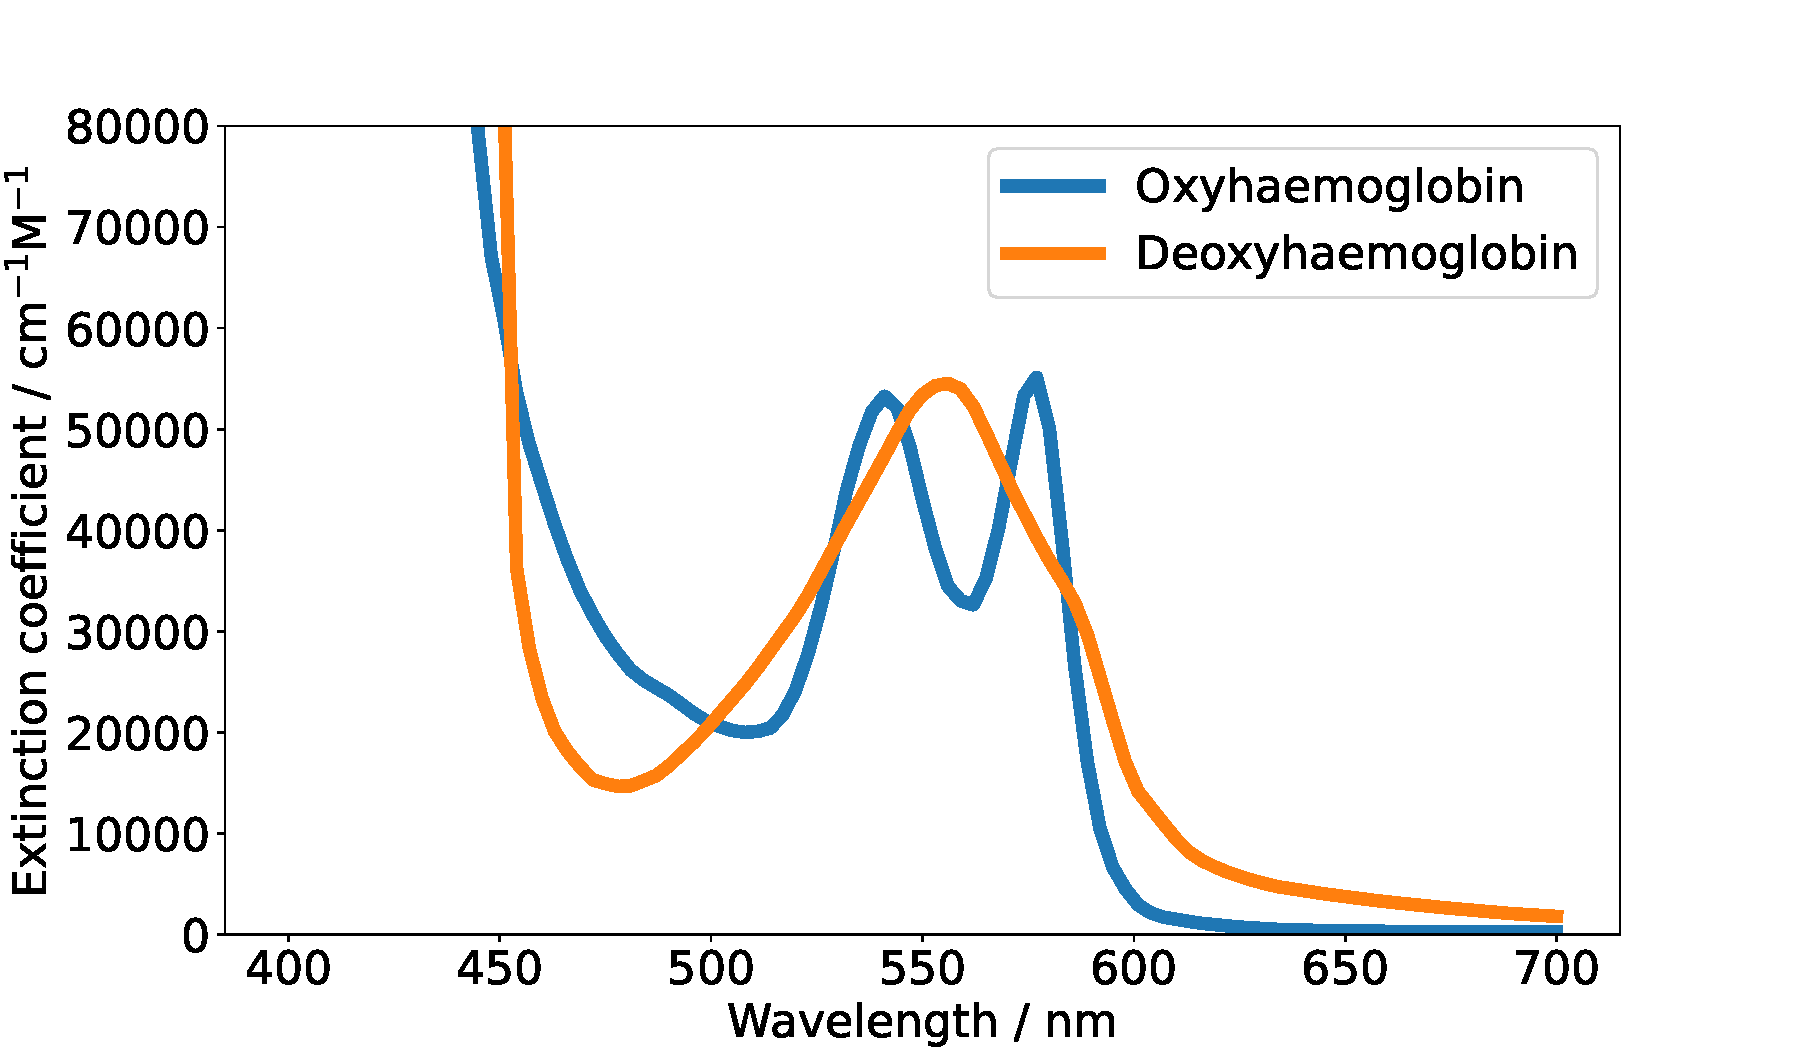
\includegraphics[width=0.7\textwidth]{Hb_eps.pdf}
    \caption{The extinction coefficients for oxyhaemoglobin and deoxyhaemoglobin reproduced from~\citenum{Prahl1998}.}
    \label{fig:Haemoglobinext}
\end{figure}
Oxygen saturation is defined as the proportion of haemoglobin which is oxygenated ie $\frac{HbO_2}{HbO_2 + Hb}$ where $Hb$ is deoxyhaemoglobin and $HbO_2$ is oxyhaemoglobin. 

There are no currently established, intra-operative, techniques to assess $StO_2$ in neurosurgery and so perfusion is often used as an indicator instead with DSA, MVD, and ICG capable of this as detailed in Sections \ref{sec:introtumourtreatments} and \ref{sec:introaneurysmtreatments}. Additionally, there has been significant research into using Laser Speckle Contrast Imaging (LSCI) to visualise blood perfusion, however this is not able to distinguish between $Hb$ and $HbO_2$~\cite{Dunn2012, Zhong2021}. Peri-operative neural monitoring can use jugular venous oxygen saturation (JVOS)~\cite{Raith2020} and cerebral oximetry~\cite{Lian2020} to provide indications of the health of the organ. Both techniques usually make use of near infra-red (NIR) spectroscopy to distinguish between $Hb$ and $HbO_2$. These techniques, however, lack specificity so local regions of ischaemia can be present when these values are within the bounds of normality~\cite{Raith2020, Zhong2021}.

Due to this lack of available techniques, there have been many proposed methods to extract $StO_2$ from tissue diffuse reflectance spectra. These range from the simplest ratiometric two-wavelength methods to more sophisticated analytical models~\cite{MacKenzie2018} or deep-learning based approaches~\cite{Ayala2023}. Using two or three wavelength models can provide good results but require data to be captured at these precise wavelengths, whereas analytical models can be applied to ranges of wavelengths for which they are developed. These analytical models also enable more detailed modelling of tissue including consideration of melanin when imaging through skin. Alternatively, Monte Carlo methods are an established approach to modelling light-tissue interaction for a range of wavelengths. It is, however, computationally challenging to apply in an inverse problem setting making the estimation of optical properties from tissue spectra non trivial on the basis of Monte Carlo simulations alone. To obtain the diffuse reflectance spectra intra-operatively, these techniques primarily use HSI which enable non-contact imaging with minimal change to surgical workflow. 

\section{Current state of the art of $StO_2$ measurement}\label{sec:stateofart}
The challenges presented in current neurosurgical practice present an interesting area for development. Many technologies are being developed to address the need for $StO_2$ assessment intra-operatively for these applications. In this section some key research technologies are presented alongside their limitations and the choice to pursue HSI in this work is justified. 

\subsection{Optical coherence tomography}
Optical Coherence Tomography (OCT) is a non-contact 3D imaging modality which provides both spatial and depth information of the tissue imaged. The technique utilises a reference beam and a sample beam; the backscattered light from the sample beam forms an interference pattern with the reference beam which is measured. Traditionally, the mirror used to produce the reference beam is adjusted until interference is maximised, and at this point the distance between the positions of the mirror and sample provides information on the depth of the scatterer. To increase efficiency, the mirror location is fixed and Fourier Transforms are used to analyse the returned interference and provide the depth of the scattering structures at the spatial location measured~\cite{Fercher2003}. By scanning the focussed beam across the sample tissue, a 3D image with both spatial and depth information can be constructed~\cite{Fercher2003}. Traditionally OCT utilises near-infrared wavelengths (NIR) due to the deeper penetration into biologically tissue, however recent advances have shown that using visible wavelengths allows oxygen saturation of vessels to be computed~\cite{Shu2017}. It has also been shown that tumour margins can be highly accurately delineated from this type of data using automated algorithms~\cite{Sunny2019}. 
%Whilst this provides spatially resolved oxygenation information of major vessels, significant attenuation is required for this calculation limiting its application to tissue directly~\cite{Shu2017}. 
This technique allows spatially-resolved, intra-operative, oxygen saturation measurement of vessels and tumour margin delineation using probes that integrate easily into the surgical workflow~\cite{Jansen2018}. Despite these key advantages of OCT, it is also associated with some significant limitations. While OCT can be adapted to measuring oxygen saturation of vessels, significant attenuation of the sample beam is required for this calculation which limits its application to tissue directly~\cite{Shu2017}. Additionally wide-field OCT obtained by scanning the focussed sample beam over the imaging area can provide good spatially-resolved information, however this is subject to motion artefacts of the tissue under examination and limits real-time wide-field implementation~\cite{Yu2015}. These limitations are significant in the context of neurosurgery where local tissue ischaemia is of significant concern and wide-field imaging provides important information for decision-making. 

\subsection{Raman spectroscopy}
Raman spectroscopy is a technique that observes wavelength shifts of laser light due to inelastic molecular scattering. These shifts correspond to vibrational modes of the scattering molecules which enables the chemical composition of the sample to be identified~\cite{Kong2015}. This technique has been combined with multivariate classification models to identify tumour margins primarily in brain and breast cancer surgeries and has recently overcome many of the challenges to its adoption including acquisition speed and accuracy~\cite{Kong2015, Fitzgerald2022}. There have also been advances in the use of this technique for oxygen saturation measurement by measuring resonant peaks of haemoglobin in the far infrared wavelengths, however this is limited to measurement of the oxygen saturation in vessels and requires calibration with blood samples of known oxygen saturation which is highly complex~\cite{TorresFilho2016}. Probe-based systems are also disruptive to surgical workflow. Despite highly accurate intra-operative tissue differentiation being achieved on a cellular level~\cite{Fitzgerald2022}, another key limitation is the lack of wide-field intra-operative applications of this technology. Finally, this technique is highly sensitive to the measurement configuration limiting its clinical application where these configurations can be highly variable. This includes the lighting used in the operating theatre which can confound the results of Raman measurements so particular attention must be paid to the design of these probes to ensure these effects are limited~\cite{Horsnell2016}, and appropriate calibrations must be used which can be disruptive to workflow~\cite{TorresFilho2016}.

\subsection{Photoacoustic imaging}
Photoacoustic imaging is a hybrid imaging modality which optically illuminates a sample, the sample then converts the optical energy to thermal energy which generates acoustic waves that are detected. Scattering of sound waves is much lower than of light in tissues so enabling deeper imaging, however increasing the depth of imaging compromises the spatial resolution~\cite{Assi2023}. By utilising different wavelengths of light, spatially-resolved $StO_2$ can be determined. This increase in the number of wavelengths used for imaging results in slower acquisition times due to the increased scanning which can result in motion artefacts in the acquired image and limiting real-time implementation~\cite{Assi2023, Attia2019}. By considering different biological or exogeneous chromophores, tumour margins can also be detected with this technique which has been primarily explored for breast cancers and melanomas~\cite{Assi2023, Attia2019, Taylor-Williams2022}. Quantitative $StO_2$ or chromophore extraction is challenging at depth due to the absorption of the incident light by chromophores in the sample, termed "spectral colouring" whose corrections often break down and biological settings~\cite{Assi2023, Taylor-Williams2022}. While some photoacoustic devices have received CE marking, many devices use high power lasers for illumination, however these come with associated risks~\cite{Assi2023}. These risks are mitigated by conforming to existing laser safety standards for eye and skin exposure, however this does not account for internal tissues, including brain tissues, that would be exposed in intra-operative use~\cite{Assi2023}. Finally, there are many different possible imaging configurations that can be used for this technology which range in ergonomics~\cite{Attia2019} and can require highly specialised training for operation~\cite{Assi2023}. Whilst photoacoustic imaging has been shown to be applicable clinically for $StO_2$ extraction, this does not provide quantitative or real-time results and many imaging configurations present challenges for intra-operative integration. 

\subsection{Probe-based diffuse reflectance spectroscopy}
When light is incident on a surface it can either be directly reflected in a specular (mirror-like) manner, or it can be internally scattered or absorbed before leaving the sample diffusely, as seen in Figure \ref{fig:diffuseR}. Specularly scattered light can carry topological information of the sample, this is examined using laser speckle spectroscopy which can investigate blood flow~\cite{Dunn2012}, however diffusely scattered light is linked to the absorption and scattering properties of the sample. 
\begin{figure}[h]
    \centering
    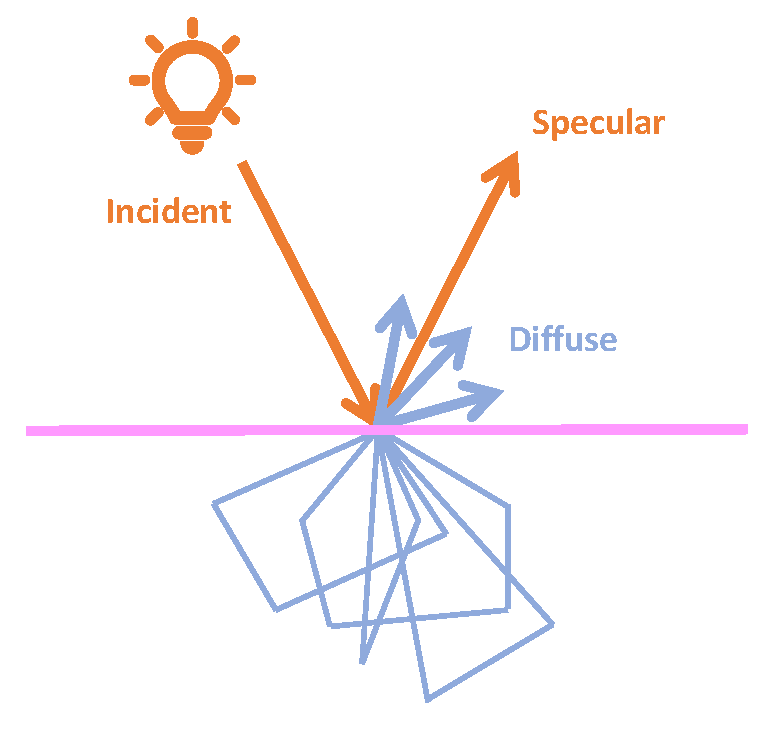
\includegraphics[width=0.4\textwidth]{Tissue_figure.pdf}
    \caption{Schematic of specularly and diffusely reflected light.}
    \label{fig:diffuseR}
\end{figure}
Diffuse reflectance spectroscopy measures this diffusely scattered light from a sample in order to gain information on the chemical composition of the sample by investigating the absorbance and scattering properties of the sample. Whilst this work focuses on HSI as a method of diffuse reflectance spectroscopy, there are many fibre-optic probe-based systems for these measurements. These systems provide highly accurate diffuse reflectance spectra in a point-based measurement. Probe-based methods are able to provide high spectral resolution measurements with short acquisition times, whereas HSI usually requires longer acquisition periods for similar spectral quality~\cite{Dinish2017}. This high spectral resolution of probe-based systems comes at the cost of spatial resolution. Whilst measurements from multiple probe locations can be stitched together~\cite{Thrapp2020}, wide-field imaging is not possible~\cite{Nishidate2015}. This technique traditionally involves contact between the probe and the sample, however this contact can alter optical properties of the tissue sample~\cite{Miller2017}. To mitigate this, flexible probes have been proposed~\cite{Miller2017} or non-contact solutions have been developed which make use of lenses and remove the impact of specular reflections using polarising filters~\cite{Bish2011, Zhu2012}. %None of these measurement configurations, however, provide wide-field information. 
Diffuse reflectance spectroscopy has shown potential for tissue differentiation~\cite{Skyrman2022} and $StO_2$ measurement~\cite{Fredriksson2020} using methods that are also applied to HSI and so are discussed more thoroughly in the following section \ref{sec:introHSI}. These techniques are able to provide real-time, intra-operative, highly accurate measurements which show promise for tissue differentiation and $StO_2$ measurement, however they do not provide wide-field imaging and non-contact configurations introduce significantly more bulk to the system. For this reason HSI is investigated to overcome these limitations. 

\subsection{Hyperspectral imaging}\label{sec:introHSI}
Hyperspectral imaging (HSI) measures diffuse reflectance spectra using multiple channels, which are narrow spectral measurements centred around a given wavelength. In comparison, traditional imaging only collects three broad channels to create a conventional RGB (red, green, blue) image. HSI provides higher spectral resolution than traditional imaging whilst maintaining a wide field of view. This technique can also be referred to as multispectral imaging when there is a low number of bands, however for simplicity we will refer to this as HSI in all cases~\cite{Clancy2020}. 

HSI is widely used in many applications and has shown promise for medical imaging~\cite{Lu2014,Giannoni2018,Calin2014,Shapey2019}. The ability to measure diffuse reflectance spectra with spatial resolution allows much more information to be displayed in a single acquisition than probe-based alternatives. This allows both spatial and spectral information to be interpretated, computationally or visually, simultaneously which may provide further insights~\cite{Seidlitz2022}. Similarly, the increased spectral resolution may allow for computation of clinically relevant physiological parameters, such as chromophore concentrations, which cannot be determined from traditional RGB imaging so reducing subjectivity~\cite{Seidlitz2022}, and enables computation for tissues directly in addition to examining vasculature. Additionally, HSI is a non-invasive, non-contact imaging modality which can be used in a compact format with minimal disruption to workflow~\cite{Thoenissen2023, Ebner2021, MacCormac2023}. Whilst there are traditionally non-sterile steps required for calibration of these measurements, we address these in Chapter \ref{chap:SWB}. Despite the increased data storage and computational requirements for the large quantities of data associated with HSI~\cite{Altamimi2022}, these advantages suggest that HSI could be a useful tool to elucidate physiological parameters intra-operatively. 

There are three major categories of HSI cameras: spatial scanning, spectral scanning, and snapshot acquisition. Spatial scanning collects data for all wavelengths simultaneously and scans through pixels sequentially, these can be sub-categorised by the scanning order such as linescan or pointscan. Spectral scanning, however, acquires data for all pixels simultaneously and scans through wavelengths sequentially. These methods both capture data consisting of two spatial and one spectral axes directly, forming a full hypercube. For both spatial and spectral scanning methods, the acquisition time is limited by the scanning time and this could lead to motion artefacts in the resulting hypercube and so snapshot implementations have been proposed to address this. The most common of these is snapshot mosaic imaging which acquires one channel per pixel in a single shot~\cite{Geelen2014} with the remaining data inferred by classical or learning-based~\cite{Li2021} interpolation (demosaicing) to construct a full hypercube. Following this demosaicing step, a spectral cross-talk correction must be performed as these systems suffer from parasitic neighbouring channel effects~\cite{Pichette2017}. This methods requires a compromise between spatial and spectral resolution where the number of spectral bands is limited in order to preserve spatial resolution. An alternative method is Coded Aperture Snapshot Spectral Imaging (CASSI) which utilises image compression tools to obtain a 2D acquisition where each pixel carries a combination of spectral and spatial information which can be decoded to produce a full hypercube measurement directly~\cite{Song2022, Eldar2009}. This method has not yet been applied intra-operatively as integration has proved challenging due to the significant increase in required optical components compared to traditional HSI approaches, and the requirement for detailed calibration of these to enable high spatial resolution reconstruction with reconstruction algorithms that are complex and computationally intensive~\cite{Song2022}. An alternative method to capture the whole hypercube in a single shot is lightfield HSI which uses a large sensor and a microarray of lenselets each with their own spectral filtering that is dependent on the angle of light. This results in an image where each pixel location corresponds to a different wavelength dependent on the lenselet projected to that position and the angle of detected light. This allows for high spectral resolution and has also shown high spatial resolution in controlled testing, however this has not yet translated to high intra-operative spectral resolution which is limited by the complex parallax correction required for a non-planar anatomical surface in addition to any motion here causing artefacts~
\cite{MacCormac2023}. Whilst I am a co-author of work integrating lightfield HSI for surgical use, this work is not presented as part of this thesis. 

Whilst spatial and spectral scanning methods have been used for most medical applications to date due to their high spectral quality, they often require long acquisition times and may be prone to motion artefacts~\cite{Kulcke2018, Giannoni2021, Shapey2019, Yoon2021}. Snapshot acquisition methods, however, allow for real-time imaging which provides improved clinical integration~\cite{Ayala2021, Ebner2021}. Since we consider spatial resolution to be of key importance for surgical guidance, we utilise snapshot mosaic imaging for this work which is depicted alongside spatial and spectral imaging methods in Figure \ref{fig:scanning}.
\begin{figure}[h]
    \centering
    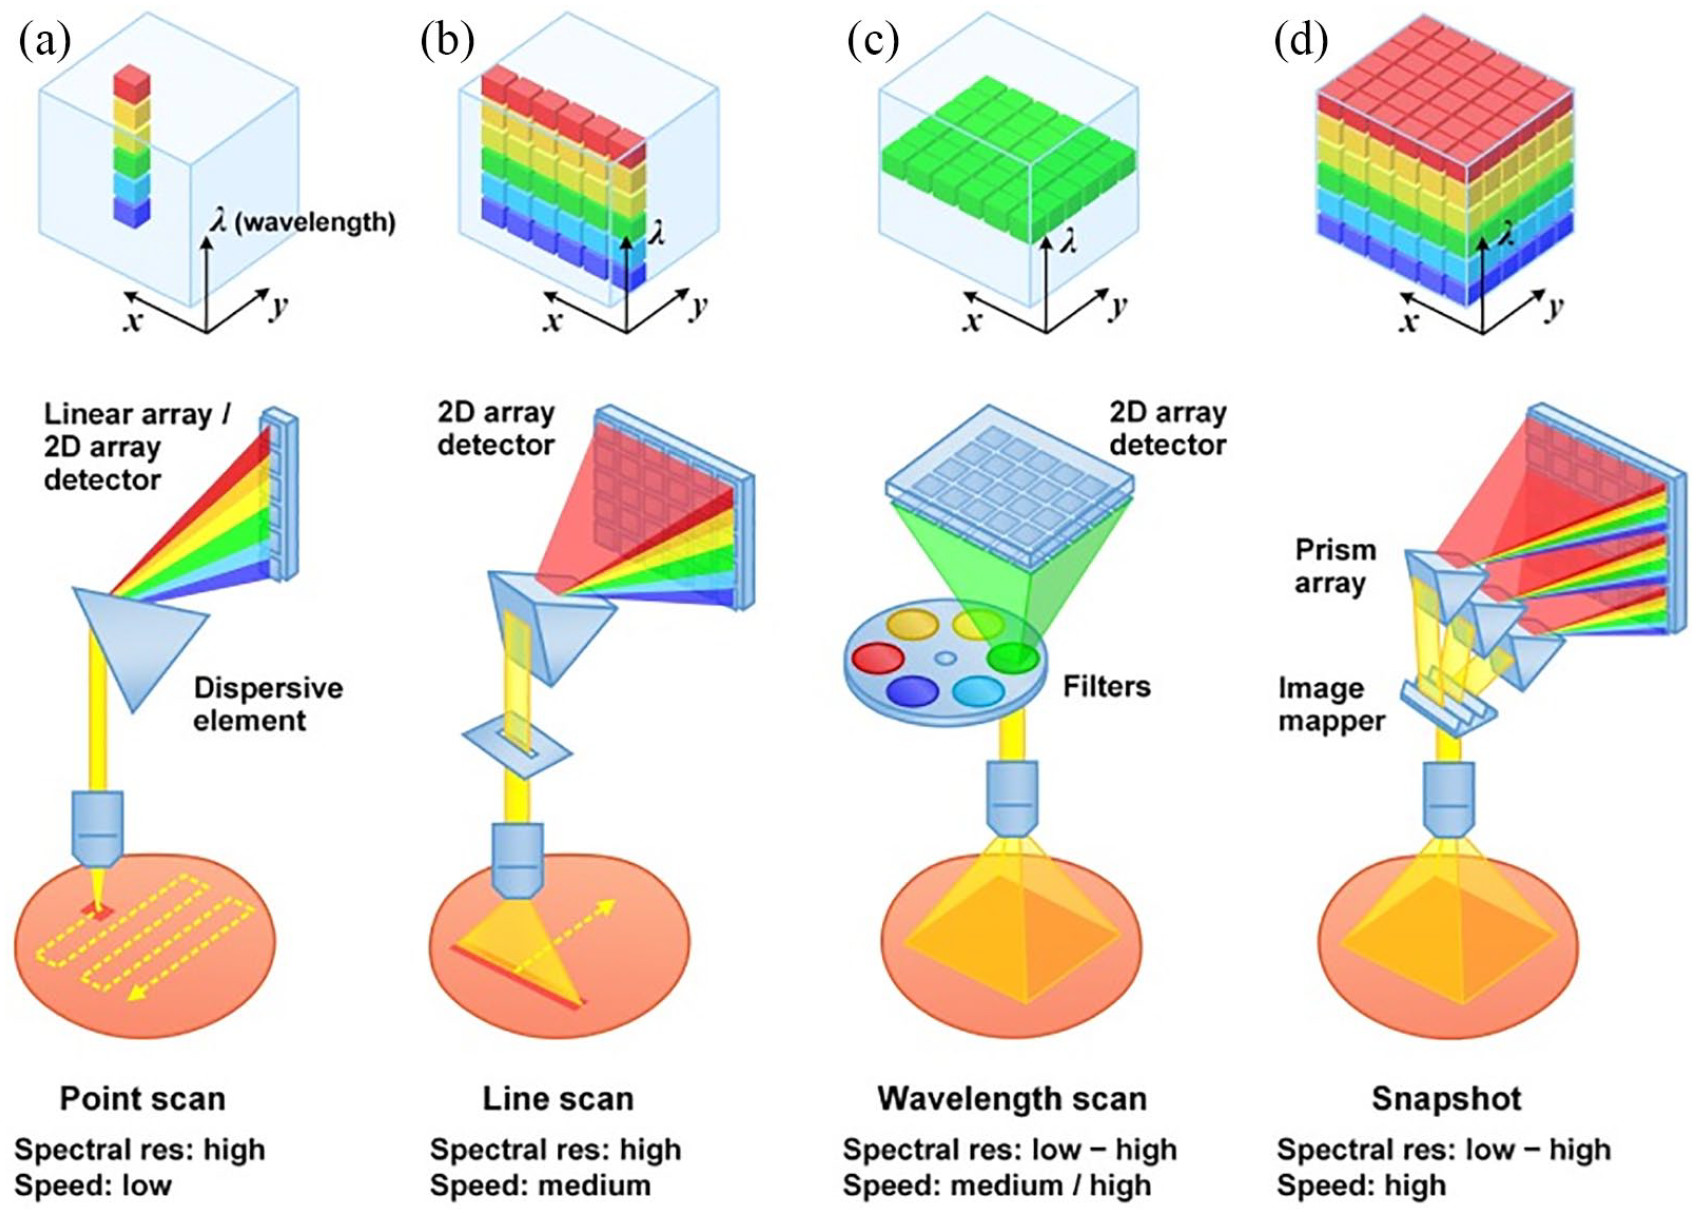
\includegraphics[width=0.7\textwidth]{scanning_types.jpeg}
    \caption{Depiction of the major HSI acquisition methods reproduced from \citenum{Araujo-Andrade2021}. Note that here the snapshot acquisition result is depicted after demosaicing.}
    \label{fig:scanning}
\end{figure}

In all cases, and traditional imaging, an initial white-balancing step must be used to account for lighting conditions, vignetting, and optical transmission through the set-up. This step traditionally uses a white and dark reference, where the white reference is an image of a uniform, highly reflective, Lambertian surface~\cite{Lu2014}. This step should be repeated for any change in imaging configuration to obtain quantitatively accurate spectral data as detailed further in Chapter \ref{chap:SWB}. Whilst these steps traditionally use non-sterile equipment and so are challenging to integrate into surgical environments, we provide a novel sterile approach in Chapter \ref{chap:SWB} to mitigate this limitation. 

Spatial Frequency Domain Imaging (SFDI) can be utilised with HSI to provide accurate, spatially-resolved, sampling depth information by projecting patterns of different frequencies which are either spatially or temporally demodulated~\cite{Gioux2019}. Whilst this provides useful additional information, for example for accurate white balancing, this method is disruptive to surgical workflow and so is not utilised in this work. 

It is hypothesised that spatially resolved, clinically relevant, physiological parameters extracted using HSI could aid decision making intra-operatively. Much investigation has already been undertaken into this with tissue differentiation~\cite{Kabwama2016, Fabelo2019, Kho2019, Giannantonio2023} and $StO_2$ extraction~\cite{Yudovsky2015, Clancy2015, WOS:000360241100026, Wirkert2016, Clancy2020, Thoenissen2023} showing great promise from intra-operative HSI data acquisition. The majority of intra-operative HSI studies have utilised spatial or wavelength scanning configurations which have integrated poorly into the surgical workflow due to the longer acquisition times~~\cite{Shapey2019, MacCormac2023, Fabelo2019}. These systems have, however, shown promising results. The HELICoiD project uses a linescan system to show intra-operative in vivo tissue differentiation with high specificity between healthy brain, tumour, and hypervascularised tissue, however this system is very bulky so integrates poorly into the surgical environment~\cite{Fabelo2019, Fabelo2019a, Kabwama2016}. \citenum{Giannantonio2023} mounted a linescan HSI camera to an operating microscope which significantly improved its integration to the surgical workflow whilst retaining the ability to differentiate tissues, however the slow acquisition time remained a limiting factor. In addition to label-free tissue differentiation, there has been growing development in the use of HSI to quantify fluorescence using 5-ALA~\cite{Walke2023}. The Tivita system uses a pointscan camera to measure a variety of parameters including $StO_2$ and has been demonstrated for assessment of wound healing viability~\cite{Thoenissen2023}, however these rely on extensive calibration and assume that the scattering contribution is wavelength-independent which may not be true for all tissues~\cite{Holmer2018, Jacques2013}. Wavelength scanning systems have also been shown to identify $StO_2$, however this application has been limited in the brain. In kidneys these studies have correlated to patient outcomes~\cite{Liu2013} but have required calibration with purely oxygenated and deoxygenated haemoglobin which is complex~\cite{Zuzak2002}. A similar system is used by \citenum{Clancy2015} for laporoscopic bowel $StO_2$ measurements without the need for complex calibrations but this assumes wavelength independent scattering functions, and \cite{Wirkert2016} however this relies on simulated training data for which it is challenging to validate experimentally. There has, however, been limited use of snapshot mosaic systems intra-operatively with \citenum{Pichette2016} being one of few to do so, however these systems provide real-time imaging potential so we choose this type of HSI system in this work. For this reason there remains the necessity to implement real-time HSI imaging with $StO_2$ modelling that sufficiently represents biological tissues with empirical validation particularly for neurosurgery. 

Throughout this thesis a snapshot HSI camera with a 4x4 mosaic pattern across the sensor (Ximea utilising the IMEC CMV2K-SSM4X4-VIS sensor, Germany) is chosen which enables fast data acquisition and integration into a variety of imaging configurations. This sensor is combined with an f=35mm coupler (Karl Storz, NDTec, VCam HD-F-35 - Camera Lens Adapter, Germany) and an exoscope (Karl Storz Endoscopy, VITOM Telescope 0° w Integ. Illuminator, UK) for imaging. This creates a standalone imaging system which is combined with various light sources. In this work, this system is used in a highly controlled manner either mounted to a seven degree of freedom robot (LBR, KUKA med7 R800, Germany) to enable multiple images to be taken with a constant reproducible camera position relative to the subject, or mounted to an optical breadboard to ensure fixed camera position, both of which can be seen in Figure \ref{fig:HSIsetups}. This system, however, is also being adapted for clinical use with the use of sterile drapes and a handheld configuration, detailed in Chapter \ref{chap:SWB}. %~\cite{Budd2023}. 
\begin{figure}[h]
    \centering 
    \begin{subfigure}[ht!]{0.27\textwidth}
	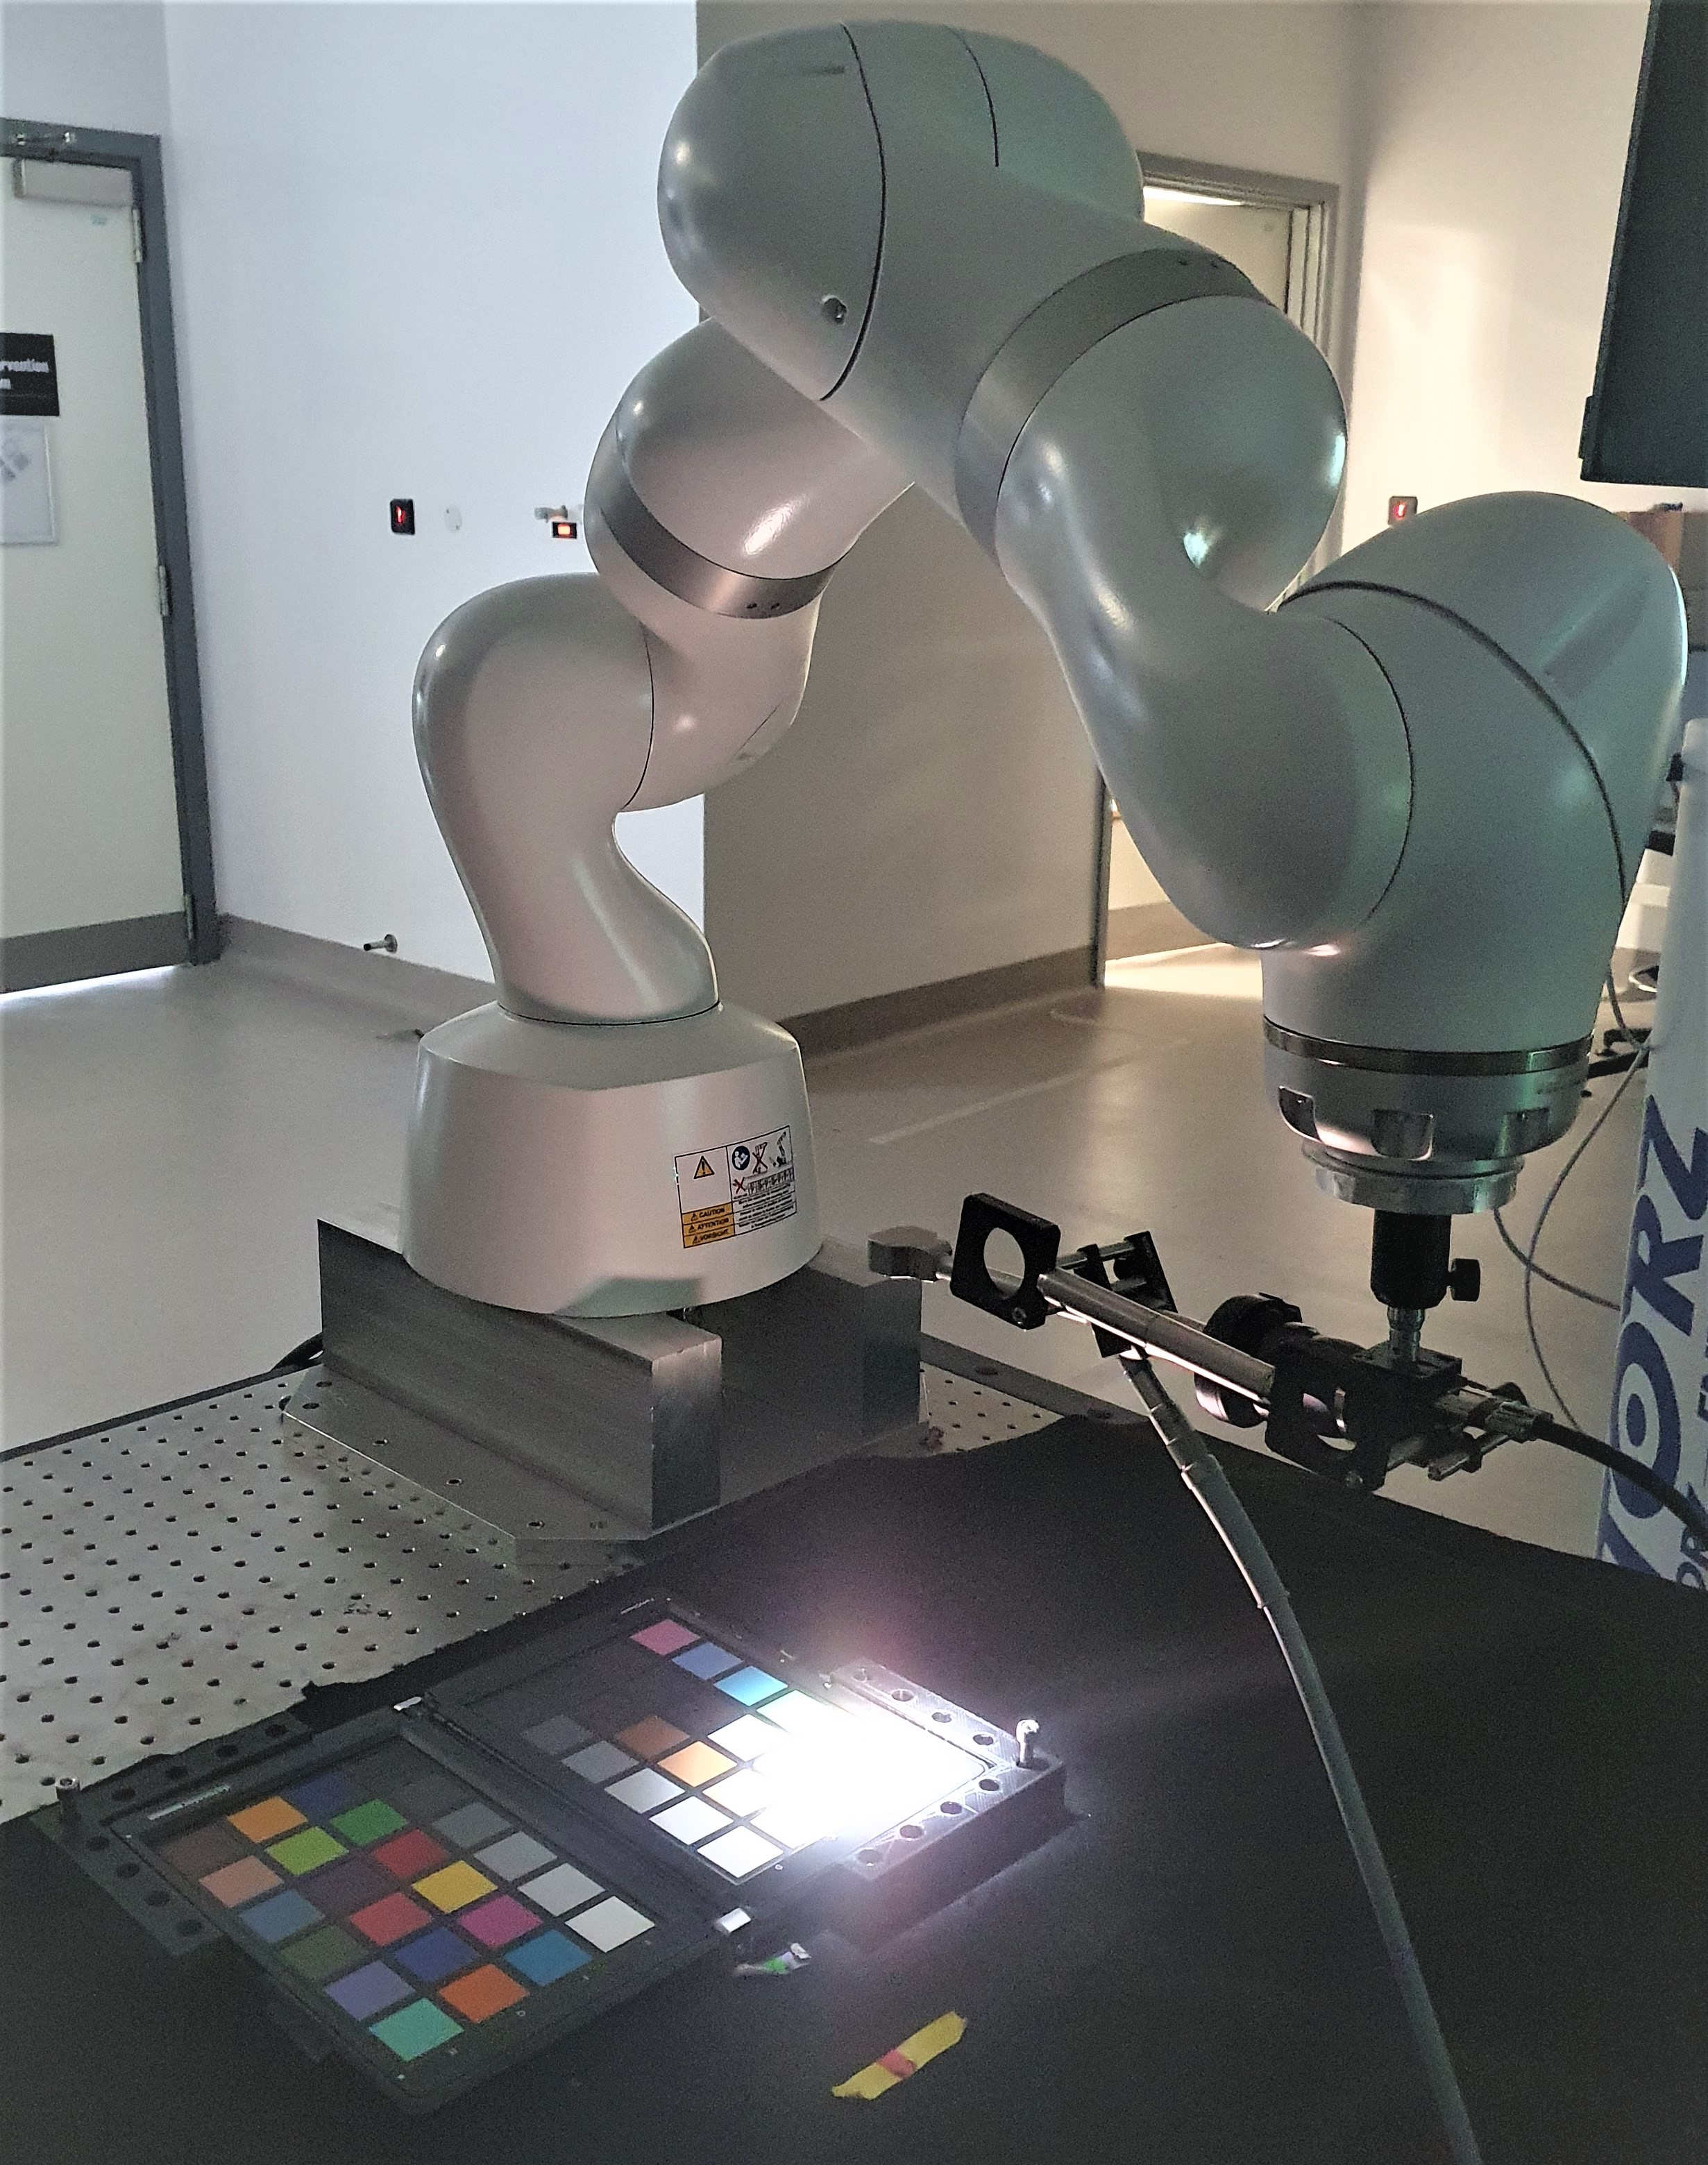
\includegraphics[width=\textwidth]{KUKAHSI}
	\caption{}
	\label{fig:KUKAHSI}
    \end{subfigure}
    \begin{subfigure}[ht!]{0.16\textwidth}
        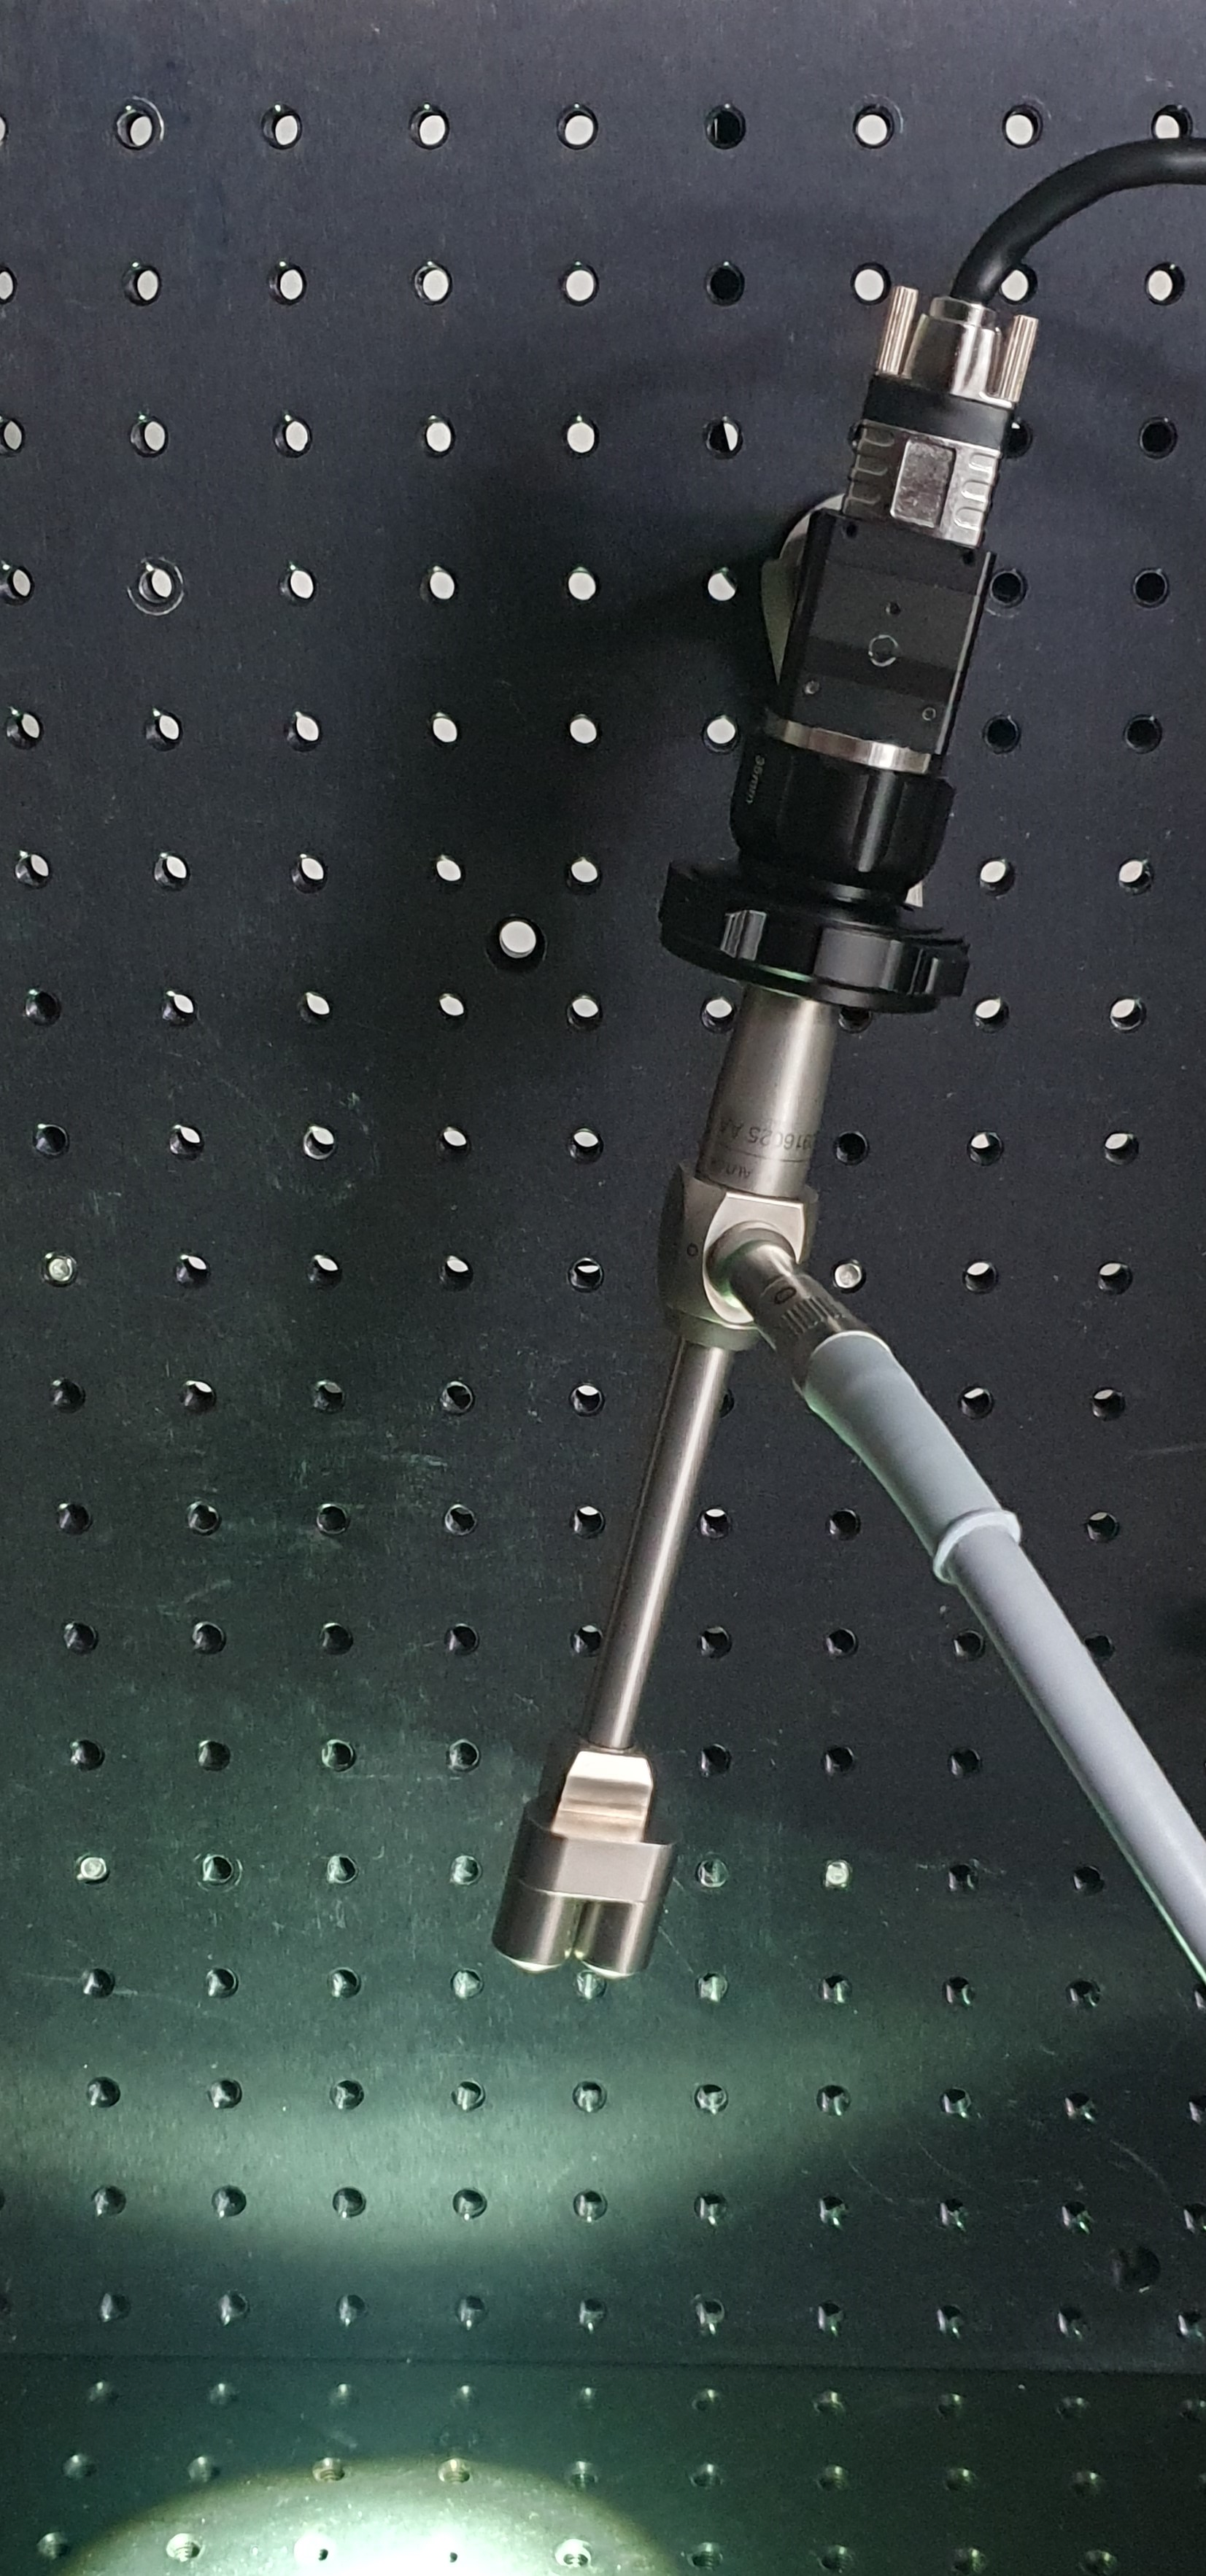
\includegraphics[width=\textwidth]{imagephantoms}
        \caption{}
        \label{fig:ScopeHSI}
    \end{subfigure}
    \caption{Snapshot HSI system comprising the sensor (Ximea utilising the IMEC CMV2K-SSM4X4-VIS sensor, Germany), an f=35mm coupler (Karl Storz, NDTec, VCam HD-F-35 - Camera Lens Adapter, Germany), and an exoscope (Karl Storz Endoscopy, VITOM Telescope 0° w Integ. Illuminator, UK) mounted to a seven degree of freedom robot (LBR, KUKA med7 R800, Germany) (\ref{fig:KUKAHSI}) or a static optical breadboard (\ref{fig:ScopeHSI}).}
    \label{fig:HSIsetups}
\end{figure}
%
%It is hoped that the increased spectral resolution would allow computation of clinically relevant physiological parameters, such as chromophore concentration. These 

\section{Outline of thesis and summary of contributions}\label{sec:thesisoutline}
In the current chapter I have outlined the principles of HSI and outlined the clinical need for an intra-operative, spatially-resolved, $StO_2$ method alongside the existing technology available for this. 
Chapter \ref{chap:SWB} investigates the necessity for in situ white references and address this by proposing a novel, sterile, synthetic reference construction algorithm. The use of references obtained at different distances and lighting conditions to the subject were examined. Spectral and color reconstructions were compared with standard measurements qualitatively and quantitatively, using $\Delta E$ and normalised RMSE respectively. The algorithm forms a composite image from a video of a standard sterile ruler, whose imperfect reflectivity is compensated for. The reference is modelled as the product of independent spatial and spectral components, and a scalar factor accounting for gain, exposure, and light intensity. Evaluation of synthetic references against ideal but non-sterile references is performed using the same metrics alongside pixel-by-pixel errors. Finally, intraoperative integration is assessed though cadaveric experiments.

Chapter \ref{chap:1layer} compares three analytical optical reflectance models for homogeneous, semi-infinite, tissue that have been proposed (Modified Beer-Lambert~\cite{Clancy2015}, Jacques 1999~\cite{Jacques1999}, Yudovsky 2009~\cite{Yudovsky2009}) which have not previously been directly compared for tissue parameter extraction purposes. I compare these analytical models using Monte Carlo simulated diffuse reflectance spectra and controlled gelatin-based phantoms with measured diffuse reflectance spectra and known ground truth composition parameters. 

In Chapter \ref{chap:2layer} a two layer model (Yudovsky 2009) is evaluated against Monte Carlo simulations and used to analyse a NIST skin reflectance dataset. By focussing on the quality of the oxygen saturation ($StO_2$) recovery, the performance of this model is evaluated across the parameter range and a significant region of failure identified. 

Chapter \ref{chap:HSImodel} investigates the impact of reducing the spectral resolution of the diffuse reflectance data and the introduction of noise by simulating camera responses from simulated and experimental data. This camera simulation is also used to adapt the analytical models for use with snapshot hyperspectral data. The impact of this is evaluated using simulations and gelatin-based phantom data similarly to previous chapters. This is evaluated using mean spectra from annotated regions of HSI images and on a pixel-by-pixel basis to investigate the ability of HSI to provide spatial resolution. Finally, some initial examples of applying these models to intra-operative, hyperspectral, neurosurgical data are shown. 